\chapter{Bayesian networks}


\section{Bayes' rule}

\begin{description}
    \item[Bayes' rule] \marginnote{Bayes' rule}
        \[ \prob{a \,\vert\, b} = \frac{\prob{b \,\vert\, a} \prob{a}}{\prob{b}} \]

    \item[Bayes' rule and conditional independence]
        Given the random variables $\texttt{Cause}$ and\\
        $\texttt{Effect}_1, \dots, \texttt{Effect}_n$, with $\texttt{Effect}_i$ independent from each other,
        we can compute $\textbf{P}(\texttt{Cause}, \texttt{Effect}_1, \dots, \texttt{Effect}_n)$ as follows:
        \[ 
            \textbf{P}(\texttt{Cause}, \texttt{Effect}_1, \dots, \texttt{Effect}_n) = 
            \left(\prod_i \textbf{P}(\texttt{Effect}_i \,\vert\, \texttt{Cause})\right) \textbf{P}(\texttt{Cause})
        \]
        The number of parameters is linear.

        \begin{example}
            Knowing that $\textbf{P} \models (\texttt{Catch} \perp \texttt{Toothache} \vert \texttt{Cavity})$:
            \[
                \begin{split}
                    \textbf{P}&(\texttt{Cavity} \,\vert\, \texttt{toothache} \land \texttt{catch}) \\
                        &= \alpha\textbf{P}(\texttt{toothache} \land \texttt{catch} \,\vert\, \texttt{Cavity})\textbf{P}(\texttt{Cavity}) \\
                        &= \alpha\textbf{P}(\texttt{toothache} \,\vert\, \texttt{Cavity})
                            \textbf{P}(\texttt{catch} \,\vert\, \texttt{Cavity})\textbf{P}(\texttt{Cavity}) \\
                \end{split}
            \]
        \end{example}
\end{description}


\section{Bayesian network reasoning}

\begin{description}
    \item[Bayesian network] \marginnote{Bayesian network}
        Graph for conditional independence assertions and a compact specification of full joint distributions.
        \begin{itemize}
            \item Directed acyclic graph.
            \item Nodes represent variables.
            \item The conditional distribution of a node is given by its parents 
                \[ \textbf{P}(X_i \,\vert\, \texttt{parents}(X_i)) \]
                In other words, if there is an edge from $A$ to $B$, then $A$ (cause) influences $B$ (effect).
        \end{itemize}

        \begin{description}
            \item[Conditional probability table (CPT)] \marginnote{Conditional probability table (CPT)}
                In the case of boolean variables, the conditional distribution of a node can be represented using 
                a table by considering all the combinations of the parents.

                \begin{example} 
                    Given the boolean variables $A$, $B$ and $C$, with $C$ depending on $A$ and $B$, we have that:\\
                    \begin{minipage}{.48\linewidth}
                        \centering
                        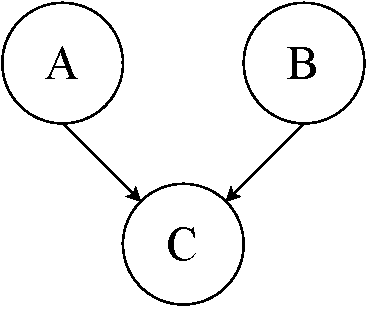
\includegraphics[width=0.35\linewidth]{img/_cpt_graph.pdf}
                    \end{minipage}
                    \begin{minipage}{.48\linewidth}
                        \centering
                        \begin{tabular}{c|c|c|c}
                            A           & B         & $\prob{c \vert A, B}$ & $\prob{\lnot c \vert A, B}$ \\
                            \hline
                            a           & b         & $\alpha$ & $1-\alpha$ \\
                            $\lnot$a    & b         & $\beta$ & $1-\beta$ \\
                            a           & $\lnot$b  & $\gamma$ & $1-\gamma$ \\
                            $\lnot$a    & $\lnot$b  & $\delta$ & $1-\delta$ \\
                        \end{tabular}
                    \end{minipage}
                \end{example}
        \end{description}

    \item[Reasoning patterns] \marginnote{Reasoning patterns}
        Given a Bayesian network, the following reasoning patterns can be used:
        \begin{descriptionlist}
            \item[Causal] \marginnote{Causal reasoning}
                To make a prediction. From the cause, derive the effect.
                \begin{example}
                    Knowing $\texttt{Intelligence}$, it is possible to make a prediction of $\texttt{Letter}$.
                    \begin{center}
                        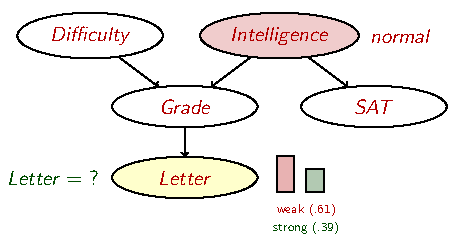
\includegraphics[width=0.5\linewidth]{img/_causal_example.pdf}
                    \end{center}
                \end{example}

            \item[Evidential] \marginnote{Evidential reasoning}
                To find an explanation. From the effect, derive the cause.
                \begin{example}
                    Knowing $\texttt{Grade}$, it is possible to explain it by estimating\\$\texttt{Intelligence}$.
                    \begin{center}
                        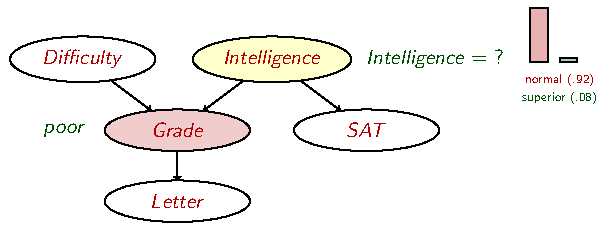
\includegraphics[width=0.7\linewidth]{img/_evidential_example.pdf}
                    \end{center}
                \end{example}

            \item[Explain away] \marginnote{Explain away reasoning}
                Observation obtained "passing through" other observations.
                \begin{example}
                    Knowing $\texttt{Difficulty}$ and $\texttt{Grade}$, 
                    it is possible to estimate \\$\texttt{Intelligence}$.

                    Note that if $\texttt{Grade}$ was not known, 
                    $\texttt{Difficulty}$ and $\texttt{Intelligence}$ would be independent.
                    \begin{center}
                        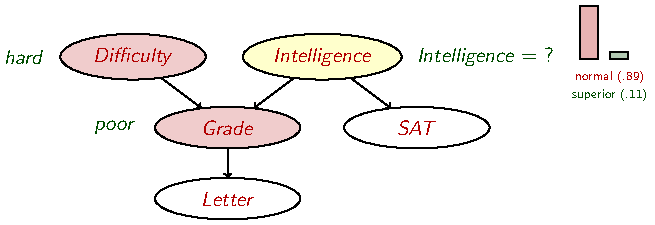
\includegraphics[width=0.75\linewidth]{img/_explainaway_example.pdf}
                    \end{center}
                \end{example}
        \end{descriptionlist}

    \item[Independence] \marginnote{Bayesian network independence}
        Intuitively, an effect is independent from a cause, 
        if there is another cause in the middle whose value is already known.
        \begin{example}
            \phantom{}

            \begin{minipage}{.3\linewidth}
                \centering
                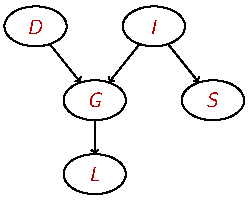
\includegraphics[width=0.85\linewidth]{img/_independence_example.pdf}
            \end{minipage}
            \begin{minipage}{.6\linewidth}
                \[ \textbf{P} \models (\texttt{L} \perp \texttt{D}, \texttt{I}, \texttt{S} \,\vert\, \texttt{G}) \]
                \[ \textbf{P} \models (\texttt{S} \perp \texttt{L} \,\vert\, \texttt{G}) \]
                \[ \textbf{P} \models (\texttt{S} \perp \texttt{D}) \text{ but } 
                    \textbf{P} \models (\texttt{S} \,\cancel{\perp}\, \texttt{D} \,\vert\, \texttt{G}) \text{ (explain away)} \]
            \end{minipage}
        \end{example}


    \item[V-structure] \marginnote{V-structure}
        Effect with two causes.
        If the effect is not in the evidence, the causes are independent.

        \begin{figure}[H]
            \centering
            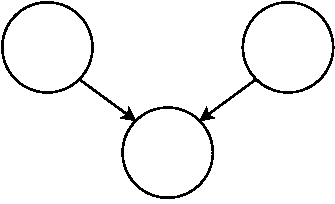
\includegraphics[width=0.2\textwidth]{img/_v_structure.pdf}
            \caption{V-structure}
        \end{figure}
    
    \item[Active two-edge trail] \marginnote{Active two-edge trail}
        The trail $X \leftrightharpoons Z \leftrightharpoons Y$ is active either if:
        \begin{itemize}
            \item $X$, $Z$, $Y$ is a v-structure $X \rightarrow Z \leftarrow Y$
                and $Z$ or one of its children is in the evidence.
            \item $Z$ is not in the evidence.
        \end{itemize}
        In other words, influence can flow from $X$ to $Y$ passing by $Z$.

        \begin{figure}[h]
            \centering
            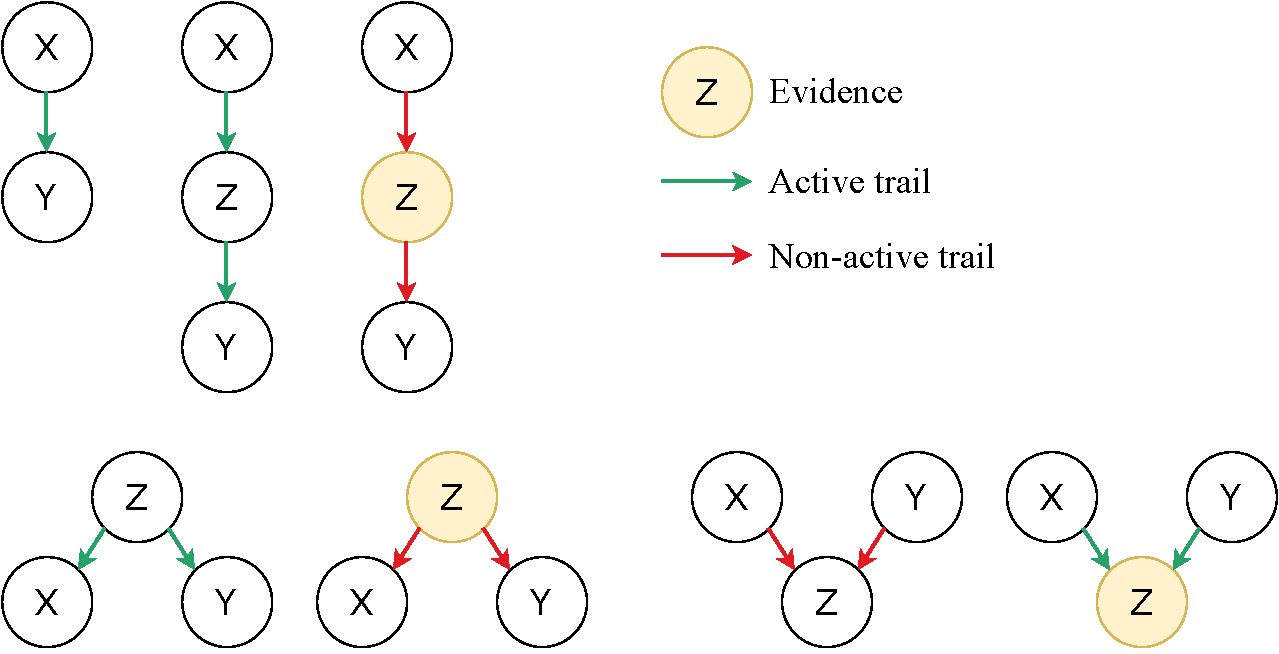
\includegraphics[width=0.65\textwidth]{img/_active_trail.pdf}
            \caption{Example of active and non-active two-edge trails}
        \end{figure}
    
    \item[Active trail] \marginnote{Active trail}
        A trail $X_1 \leftrightharpoons \dots \leftrightharpoons X_n$ is active iff
        each two-edge trail $X_{i-1} \leftrightharpoons X_i \leftrightharpoons X_{i+1}$ along the trail is active.

    \item[D-separation] \marginnote{D-separation}
        Two sets of nodes $\vec{X}$ and $\vec{Y}$ are d-separated given the evidence $\vec{Z}$ if
        there is no active trail between any $X \in \vec{X}$ and $Y \in \vec{Y}$.

        \begin{theorem}
            Two d-separated nodes are independent.
            In other words, two nodes are independent if there is no active trail between them.
        \end{theorem}

    \item[Independence algorithm] \phantom{}
        \begin{description}
            \item[Blocked node]
                A node is blocked if it blocks the flow.
                This happens if one and only one of the following conditions are met:
                \begin{itemize}
                    \item The node is in the middle of an unmarked v-structure.
                    \item The node is in the evidence.
                \end{itemize}
        \end{description}
        To determine if $X \perp Y$ given the evidence $\vec{Z}$:
        \begin{enumerate}
            \item Traverse the graph bottom-up marking all nodes in $\vec{Z}$ or
                having a child in $\vec{Z}$.
            \item Find a path from $X$ to $Y$ that does not pass through a blocked node.
            \item If $Y$ is not reachable from $X$, then $X$ and $Y$ are independent.
                Otherwise $X$ and $Y$ are dependent.
        \end{enumerate}

        \begin{example}
            To determine if $J \perp D$:
            \begin{center}
                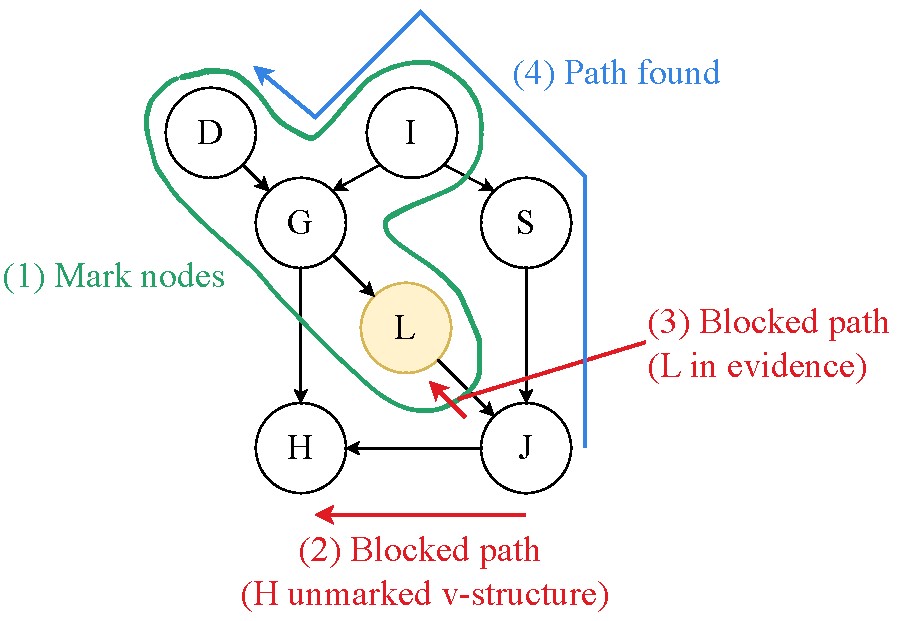
\includegraphics[width=0.5\textwidth]{img/_d_sep_example.pdf}
            \end{center}
            As a path has been found, $J \,\cancel{\perp}\, D$.
        \end{example}
    

    \item[Global semantics] \marginnote{Global semantics}
        Given a Bayesian network, the full joint distribution can be defined as
        the product of the local conditional distributions:
        \[ \prob{x_1, \dots, x_n} = \prod_{i=1}^{n} \prob{x_i \,\vert\, \texttt{parents}(X_i)} \]

        \begin{example}
            Given the following Bayesian network:

            \begin{minipage}{.3\linewidth}
                \centering
                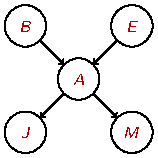
\includegraphics[width=0.7\linewidth]{img/_global_semantics_example.pdf}
            \end{minipage}
            \begin{minipage}{.6\linewidth}
                \[ 
                    \begin{split}
                        &\prob{j \land m \land a \land \lnot b \land \lnot e} \\
                            &= \prob{\lnot b} \prob{\lnot e} \prob{a \,\vert\, \lnot b, \lnot e}
                                \prob{j \,\vert\, a} \prob{m \,\vert\, a}
                    \end{split}
                \]
            \end{minipage}
        \end{example}

    \item[Local semantics]
        Each node is conditionally independent of its non-descendants given its parents.
        \begin{figure}[h]
            \centering
            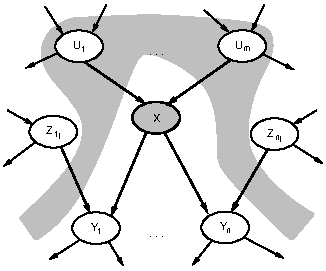
\includegraphics[width=0.35\textwidth]{img/_local_independence.pdf}
            \caption{Local independence}
        \end{figure}

        \begin{theorem}
            Local semantics $\iff$ Global semantics
        \end{theorem}
        
    
    \item[Markov blanket]
        Each node is conditionally independent of all other nodes 
        if its Markov blanket (parents, children, children's parents) is in the evidence.
        \begin{figure}[h]
            \centering
            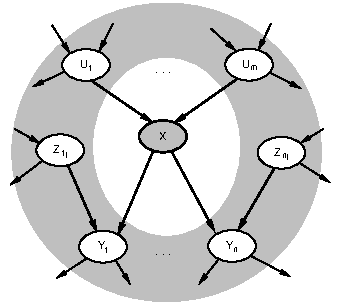
\includegraphics[width=0.35\textwidth]{img/_markov_blanket.pdf}
            \caption{Markov blanket}
        \end{figure}
\end{description}



\section{Building Bayesian networks}

\subsection{Algorithm}
The following algorithm can be used to construct a Bayesian network of $n$ random variables:
\begin{enumerate}
    \item Choose an ordering of the variables $X_1, \dots, X_n$.
    \item For $i=1, \dots, n$:
        \begin{itemize}
            \item Add $X_i$ to the network.
            \item Select the parents of $X_i$ from $X_1, \dots, X_{i-1}$ such that:
                \[ \textbf{P}(X_i \,\vert\, \texttt{parents}(X_i)) = 
                    \textbf{P}(X_i \,\vert\, X_1, \dots, X_{i-1}) \]
        \end{itemize}
\end{enumerate}
By construction, this algorithm guarantees the global semantics.

\begin{example}[Monty Hall]
    The variables are:
    \begin{itemize}
        \item $G$: the choice of the guest.
        \item $H$: the choice of the host.
        \item $P$: the position of the prize.
    \end{itemize}
    Note that $P \perp G$.
    Let the order be fixed as follows: $P$, $G$, $H$.

    \begin{figure}[h]
        \begin{subfigure}{.3\textwidth}
            \centering
            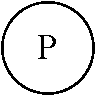
\includegraphics[width=0.15\linewidth]{img/_monty_hall1.pdf}
            \caption{First interaction}
        \end{subfigure}
        \begin{subfigure}{.3\textwidth}
            \centering
            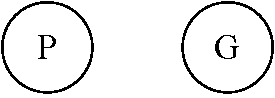
\includegraphics[width=0.45\linewidth]{img/_monty_hall2.pdf}
            \caption{Second interaction (note that $P \perp G$)}
        \end{subfigure}
        \begin{subfigure}{.3\textwidth}
            \centering
            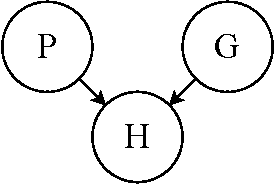
\includegraphics[width=0.45\linewidth]{img/_monty_hall3.pdf}
            \caption{Third interaction}
        \end{subfigure}
    \end{figure}
\end{example}

The nodes of the resulting network can be classified as:
\begin{descriptionlist}
    \item[Initial evidence] The initial observation.
    \item[Testable variables] Variables that can be verified.
    \item[Operable variables] Variables that can be changed by intervening on them.
    \item[Hidden variables] Variables that "compress" more variables to reduce the parameters.
\end{descriptionlist}

\begin{example} \phantom{}\\
    \begin{minipage}{.4\linewidth}
        \begin{description}
            \item[Initial evidence] Red.
            \item[Testable variables] Green.
            \item[Operable variables] Orange.
            \item[Hidden variables] Gray.
        \end{description}
    \end{minipage}
    \begin{minipage}{.5\linewidth}
        \begin{center}
            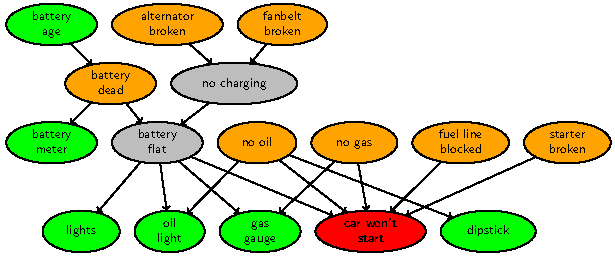
\includegraphics[width=\linewidth]{img/_car_example.pdf}
        \end{center}
    \end{minipage}
\end{example}


\subsection{Structure learning}
\marginnote{Structure learning}
Learn the network from the available data.
\begin{description}
    \item[Constraint-based] 
        Independence tests to identify the constraints of the edges.
    \item[Score-based] 
        Define a score to evaluate the network.
\end{description}



\section{Causal networks}
When building a Bayesian network, a correct ordering of the nodes 
that respects the causality allows to obtain more compact networks.

\begin{description}
    \item[Structural equation] \marginnote{Structural equation}
        Given a variable $X_i$ with values $x_i$, its structural equation is a function $f_i$
        such that it represents all its possible values:
        \[ x_i = f_i(\text{other variables}, U_i) \]
        $U_i$ represents unmodeled variables or error terms.

    \item[Causal network] \marginnote{Causal network}
        Restricted class of Bayesian networks that only allows causally compatible ordering.

        An edge exists between $X_j \rightarrow X_i$ iff $X_j$ is an argument of 
        the structural equation $f_i$ of $X_i$.

        \begin{example} \phantom{}\\[0.5em]
            \begin{minipage}{.3\linewidth}
                \centering
                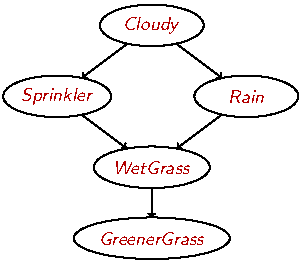
\includegraphics[width=\linewidth]{img/_causal_network_example1.pdf}
            \end{minipage}
            \begin{minipage}{.6\linewidth}
                The structural equations are:
                \[ 
                    \begin{split}
                        \texttt{cloudy} &= f_C(U_C) \\
                        \texttt{sprinkler} &= f_S(\texttt{Cloudy}, U_S) \\
                        \texttt{rain} &= f_R(\texttt{Cloudy}, U_R) \\
                        \texttt{wet\_grass} &= f_W(\texttt{Sprinkler}, \texttt{Rain}, U_W) \\
                        \texttt{greener\_grass} &= f_G(\texttt{WetGrass}, U_G)
                    \end{split}
                \]
            \end{minipage}\\[0.5em]

            If the sprinkler is disabled, the network becomes:\\[0.5em]
            \begin{minipage}{.3\linewidth}
                \centering
                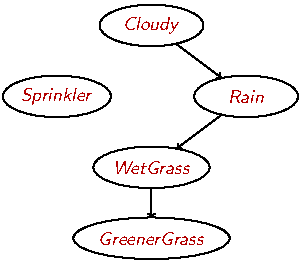
\includegraphics[width=\linewidth]{img/_causal_network_example2.pdf}
            \end{minipage}
            \begin{minipage}{.6\linewidth}
                The structural equations become:
                \[ 
                    \begin{split}
                        \texttt{cloudy} &= f_C(U_C) \\
                        \texttt{sprinkler} &= f_S(U_S) \\
                        \texttt{rain} &= f_R(\texttt{Cloudy}, U_R) \\
                        \texttt{wet\_grass} &= f_W(\texttt{Rain}, U_W) \\
                        \texttt{greener\_grass} &= f_G(\texttt{WetGrass}, U_G)
                    \end{split}
                \]
            \end{minipage}
        \end{example}

    \item[do-operator] \marginnote{do-operator}
        The do-operator allows to represent manual interventions on the network.
        The operation $\texttt{do}(X_i = x_i)$ makes the structural equation of $X_i$
        constant (i.e. $f_i = x_i$, without arguments, so there won't be inward edges to $X_i$).

        \begin{example} \phantom{}\\[0.5em]
            \begin{minipage}{.3\linewidth}
                \centering
                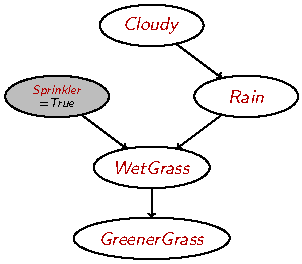
\includegraphics[width=\linewidth]{img/_do_operator_example1.pdf}
            \end{minipage}
            \begin{minipage}{.65\linewidth}
                By applying $\texttt{do}(\texttt{Sprinkler} = \texttt{true})$, the structural equations become:
                \[ 
                    \begin{split}
                        \texttt{cloudy} &= f_C(U_C) \\
                        \texttt{sprinkler} &= \texttt{true} \\
                        \texttt{rain} &= f_R(\texttt{Cloudy}, U_R) \\
                        \texttt{wet\_grass} &= f_W(\texttt{Sprinkler}, \texttt{Rain}, U_W) \\
                        \texttt{greener\_grass} &= f_G(\texttt{WetGrass}, U_G)
                    \end{split}
                \]
            \end{minipage}\\[0.5em]

            \begin{minipage}{.3\linewidth}
                \centering
                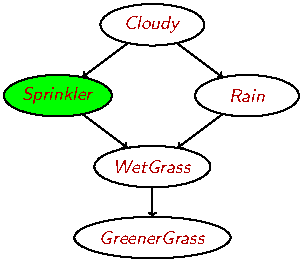
\includegraphics[width=\linewidth]{img/_do_operator_example2.pdf}
            \end{minipage}
            \begin{minipage}{.65\linewidth}
                Note that Bayesian networks are not capable of modelling manual interventions.
                In fact, intervening and observing a variable are different concepts:
                \[ \prob{\texttt{WetGrass} \mid \texttt{do}(\texttt{Sprinkler} = \texttt{true})} \]
                \[ \neq \]
                \[ \prob{\texttt{WetGrass} \mid \texttt{Sprinkler} = \texttt{true}} \]
            \end{minipage}
        \end{example}
\end{description}